\section{Interfaz}

La interfaz es la siguiente:

\begin{figure}[H]
   \centering
   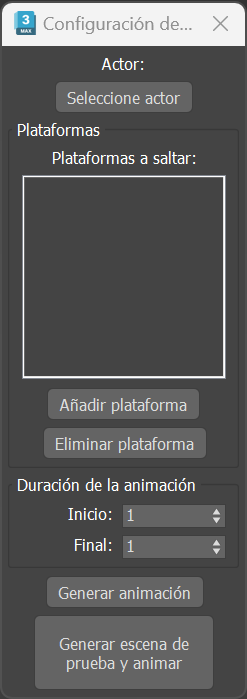
\includegraphics[width=0.2\textwidth]{imagenes/ui1.png}
   \caption{Interfaz del programa.}
\end{figure}

Como se puede ver, aparece un primer botón para elegir el objeto que será animado.

\bigskip

A continuación aparece una lista, junto a dos botones para añadir plataformas o eliminarlas. Conforme se van añadiendo, la lista va creciendo. Además, si se pulsa sobre una de las plataformas de la lista y se le da al botón de eliminar, desaparece de la lista y no se tendrá en cuenta en la animación.

\bigskip

Después, aparece la parte del \textit{timeline}, donde se puede elegir el instante de inicio y de finalización de la animación.

\bigskip

Finalmente aparece el botón de generar la animación, que solo se ejecutará si todo está correctamente elegido.

\bigskip

Como he dicho antes, para asegurarme de que todo esté bien configurado he añadido comprobaciones para no poder elegir el mismo objeto como el que vaya a saltar y como plataforma. Asimismo, he puesto otras como: comprobación de que haya al menos dos plataformas, comprobación de que el tiempo de inicio sea menor que el de finalización y comprobación de que se ha elegido un objeto para animar.

\bigskip
\newpage

A continuación muestro algunos errores que pueden salir:

\begin{figure}[H]
\begin{subfigure}[t]{0.48\textwidth}
    \centering
    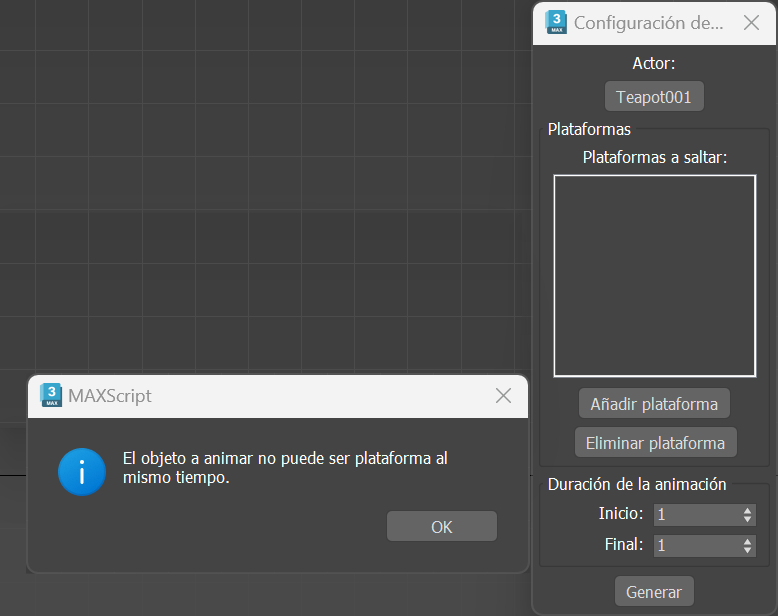
\includegraphics[width=\textwidth]{imagenes/error1.png}
    \caption{Error de un mismo objeto como actor y plataforma.}
 \end{subfigure}
\hfill
 \begin{subfigure}[t]{0.48\textwidth}
    \centering
    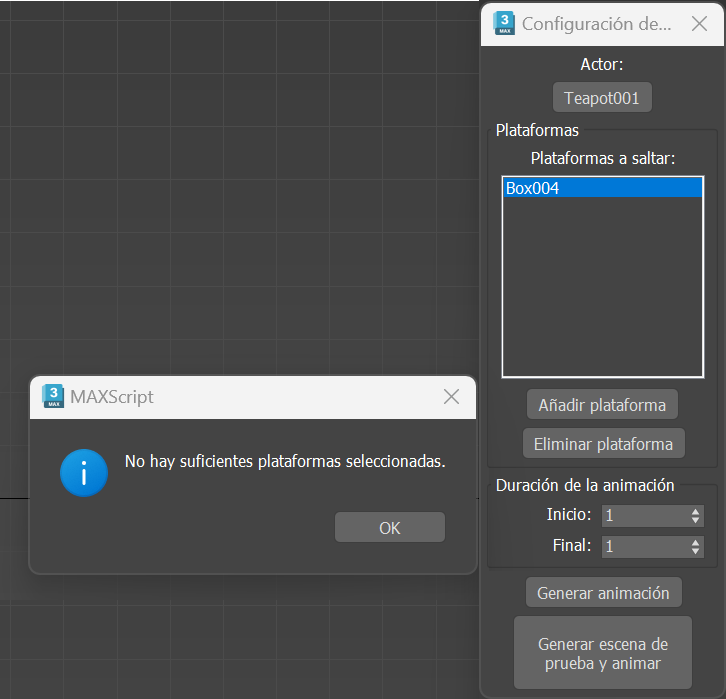
\includegraphics[width=\textwidth]{imagenes/error2.png}
    \caption{Error de no haber suficientes plataformas.}
 \end{subfigure}
\par\bigskip
\begin{subfigure}[t]{\textwidth}
    \centering
    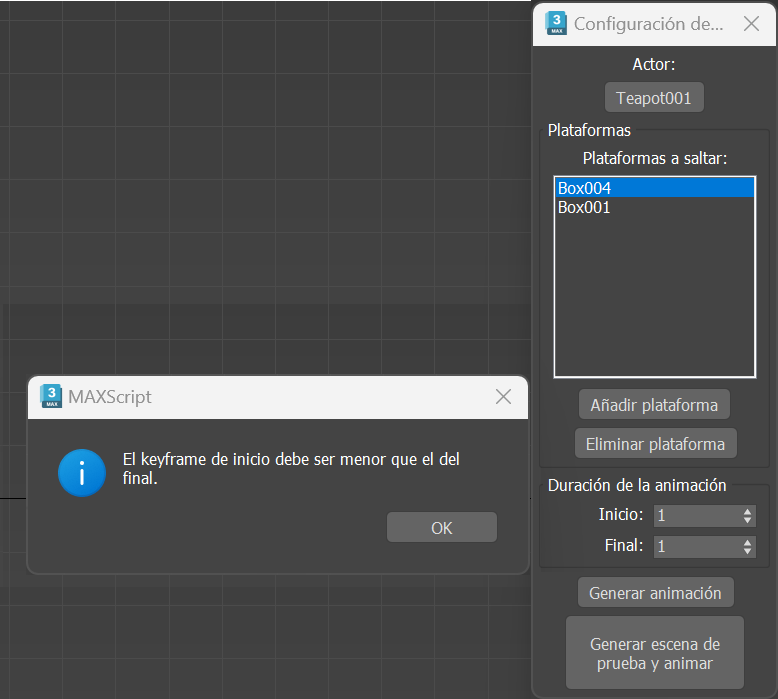
\includegraphics[width=0.48\textwidth]{imagenes/error3.png}
    \caption{Error de intervalo de animación inválido.}
 \end{subfigure}
 \caption{Pantallas con los distintos avisos que puede dar el programa.}
\end{figure}

\newpage

Y un ejemplo de configuración correcta de la interfaz es:

% imagen de la interfaz rellena

\begin{figure}[H]
    \centering
    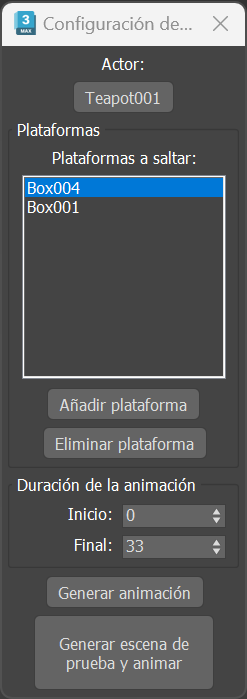
\includegraphics[width=0.2\textwidth]{imagenes/ui2.png}
    \caption{Interfaz con los datos rellenos correctamente.}
 \end{figure}